% !TeX spellcheck = en_US
% !TeX root = notes.tex
\section{Lecture 2: Bitcoin, Cryptocurrencies Blockchain Technology}
Blockchain is over-hyped!
\subsection{Blockchain (or Hash Chain/List)}
\begin{itemize}
	\item Use hash pointers to build structures similar to a linked list
	\item Head hash pointer of the list protects the integrity of the entire list or chain (Need to store hash pointer to the head of the list externally to list)
	\item Hash is computed over entire block, including header, which includes hash pointer to previous block
	\item First block is called \textbf{Genesis Block}
	\item If an attacker modifies a block, they need to modify the contents of all subsequent blocks
\end{itemize}
\subsubsection{Merkle Trees}
\begin{note}{Merkle Trees}
	\begin{itemize}
		\item Named after Ralph Merkle
		\item Can protect integrity of large number of data blocks, like a Blockchain
		\item We only need the \textbf{Root Hash} at the root of the tree (\textbf{Merkle Root})
		\item Modification of any data block by attack results in different hashes all the way up to the Merkle Root, and can easily be detected
		\item Cost to prove \texttt{Tx1} in the tree: $O(\log_2 N)$
	\end{itemize}
\end{note}
\begin{figure}[H]
	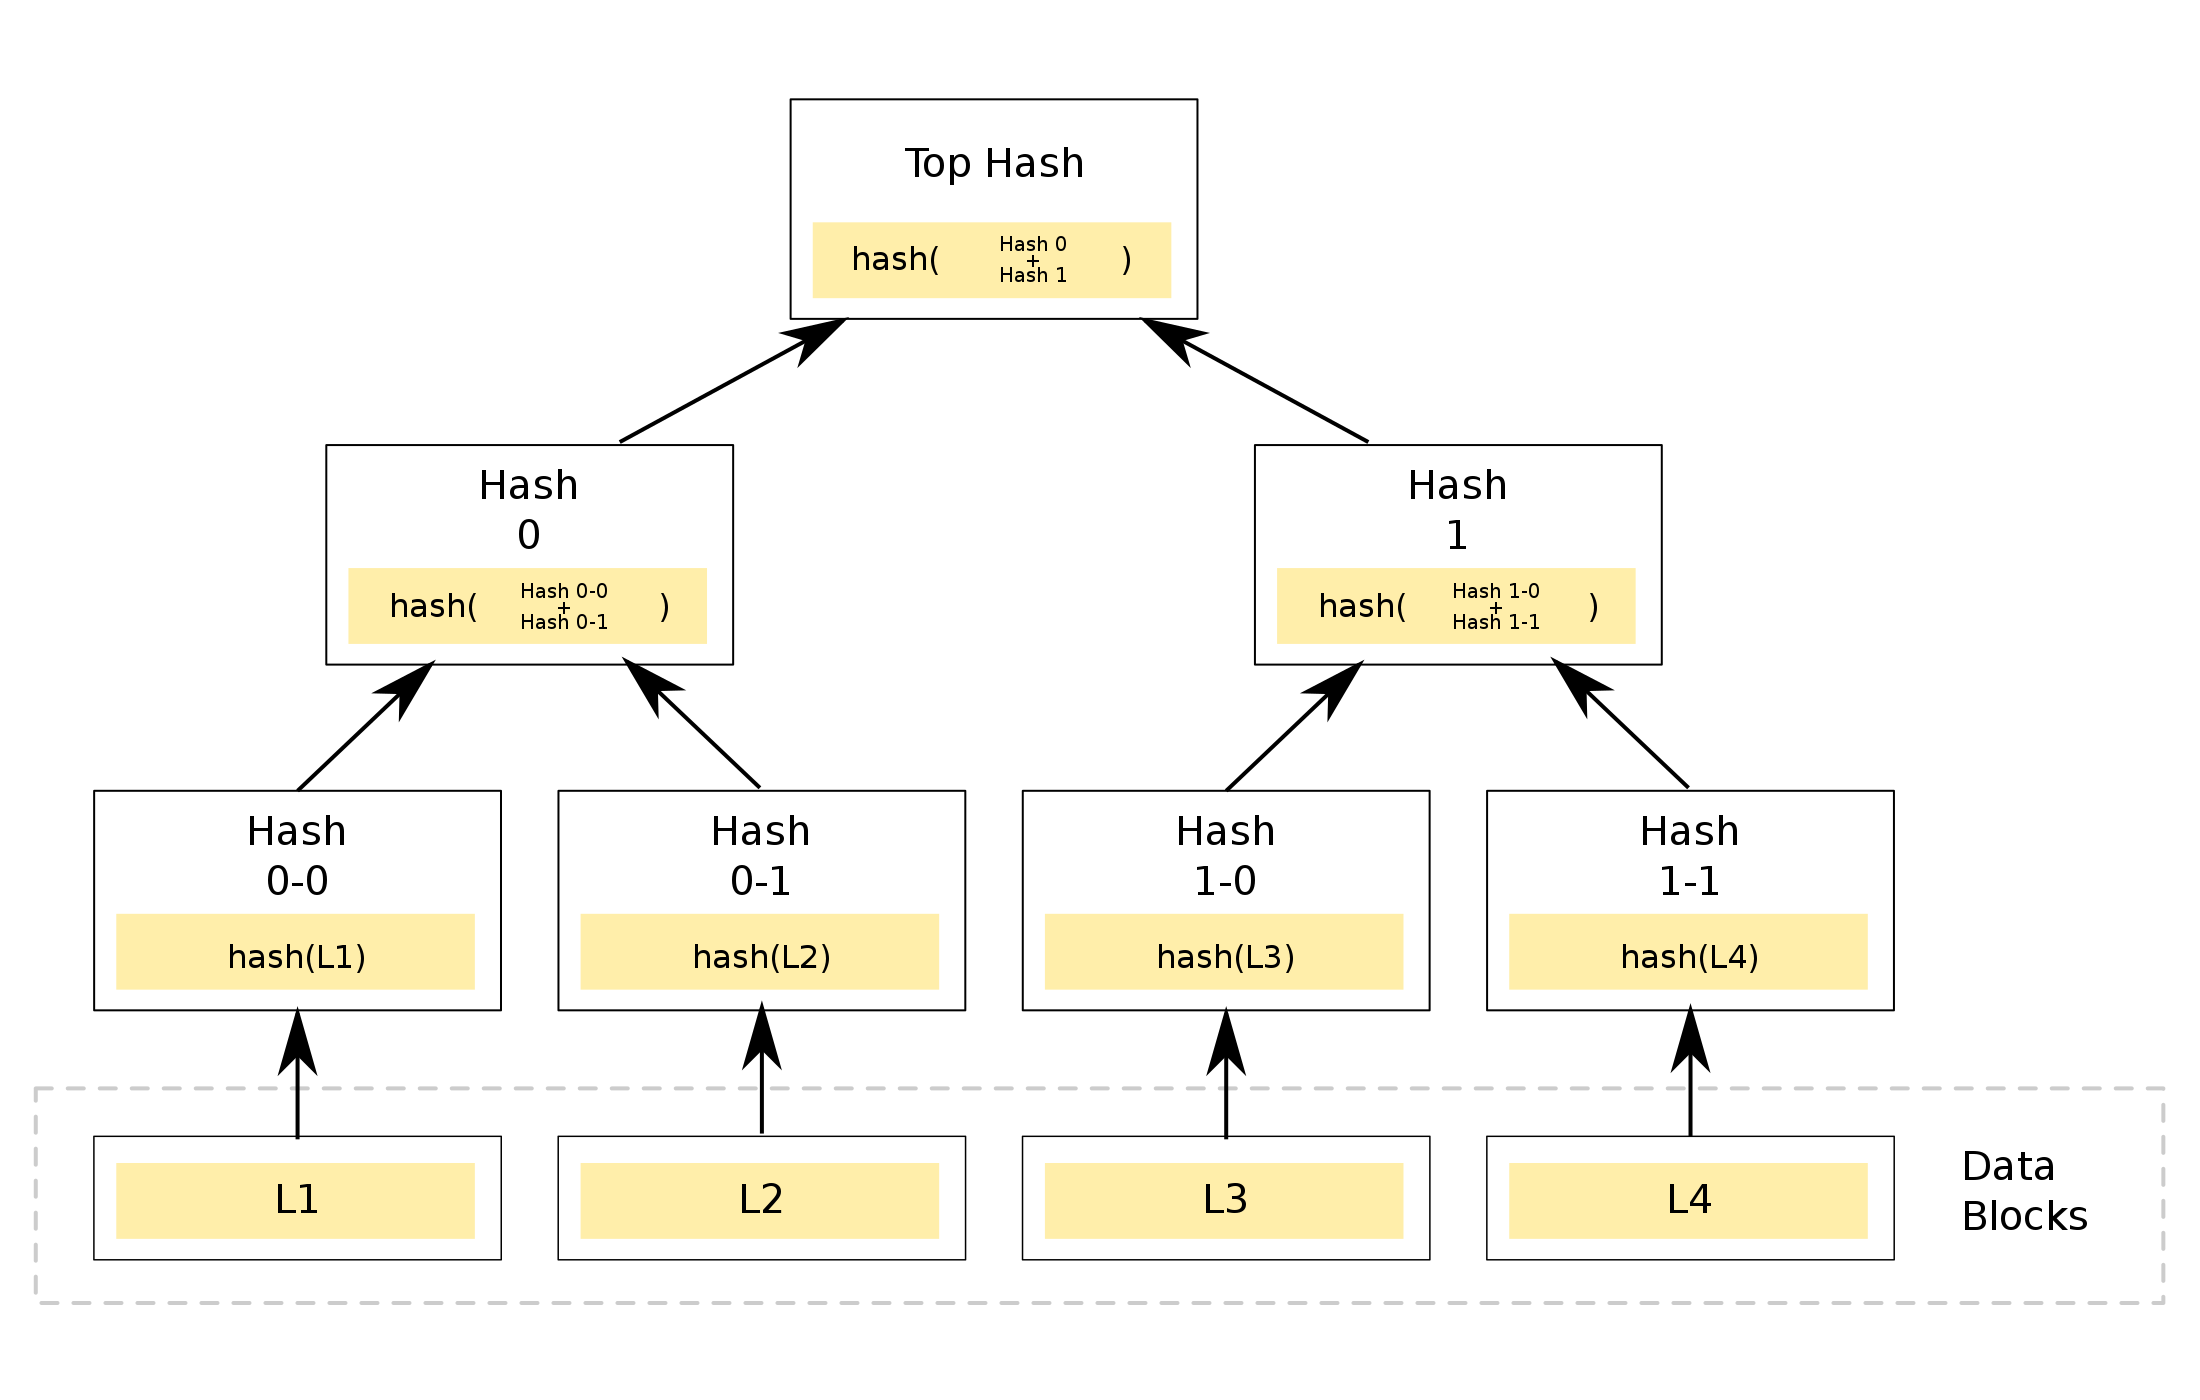
\includegraphics[width=\linewidth]{merkle}
	\centering
	\caption{Merkle Tree Layout}
\end{figure}
\subsubsection{Use of Merkle Trees in Bitcoin}
Bitcoin uses Merkle Trees to store Transactions in a ``Block'' ($\approx2000$)
\begin{itemize}
	\item Each Block stores a \textbf{Merkle Root}
	\item Merkle Trees allow verification that a transaction is part of a Block without having the entire block, only Merkle Path is required. This is used to implement Simplified Payment Verification (SPV) in Bitcoin
\end{itemize}
Blocks are then stored in a Blockchain

\subsection{Public Key Cryptography -- Digital Signatures}
Properties of signatures
\begin{itemize}
	\item Only \textbf{you} can provide a valid signature, anyone can verify
	\item Signature is tied to a particular document, cannot be copy-pasted to another document
\end{itemize}
Public Key Cryptography
\begin{itemize}
	\item Asymmetric operation
	\item Two keys: Public key and Private key
\end{itemize}
Encryption
\begin{itemize}
	\item Encryption with Public Key
	\item Decryption with Private Key
	\item Key Benefit: Simplified key distribution/management
	\item Remaining security problems $\rightarrow$ Authenticity of public key, Public Key Certificates (map public key to identity)
\end{itemize}
Digital Signature
\begin{itemize}
	\item Sign with Private Key
	\item Verification with Public Key
\end{itemize}
\begin{leftbar}
	Since public key operations are computationally expensive, digital signatures are typically applied to a hash, rather than entire file or block of data
\end{leftbar}
\subsubsection{Digital Signatures in Bitcoin}
Bitcoin transactions have digital signatures
\begin{itemize}
	\item Signed by the owner(s) of the source funds (Bitcoin to be transferred)
	\item This proves ownership of funds
	\item Prevents forgery of coins/transactions
\end{itemize}
\begin{note}{Bitcoin Identity}
	An identity in Bitcoin (a \textbf{Bitcoin Address}) is simply a public key (160-bit hash of it, to be precise)
	\begin{itemize}
		\item No need for public key certificates
		\item No need to link public key to a real name
	\end{itemize}
\end{note}

\subsubsection{Hashcash}
\begin{note}{Hashcash}
	Prevent of mitigate \textbf{denial-of-service} (DoS) attacks by requiring the sender to solve a puzzle before connecting
	\begin{sequencediagram}
		\newinst{c}{Client}
		\newinst[3]{s}{Server}
		
		\mess{c}{Request Service}{s}
		\mess{s}{Choose Challenge}{s}
		\mess{s}{Send Challenge}{c}
		\mess{c}{Solve}{c}
		\mess{c}{Response}{s}
		\mess{s}{Verify}{s}
		\mess{s}{Grant Service}{c}
	\end{sequencediagram}
\end{note}
\begin{itemize}
	\item Require the first $n$ bits of $h(x)$ to have a given value, first $n$ bits are all $0$ (partial pre-image)
	\item Same as saying $h(x) < T$
	\item Best approach is brute forcing
	\item Chance of guessing on single try: $2^{-n}$, expected number of tries until success: $2^n$
\end{itemize}
\textit{Bitcoin aims to have a block solved roughly every 10 minutes, difficulty is adjusts every 2016 blocks ($\approx2$ weeks)}

\subsection{Cryptocurrency}
\begin{description}
	\item[Broadcasting of transactions:] Unstructured P2P Network, flooding (as used in Bitcoin)
	\item[Avoiding forgery (transactions, coins):] Digital Signatures
	\item[Maintaining the public ledger:] P2P Network, Proof-of-work and Incentive mechanism
\end{description}